\documentclass{beamer}
\usetheme{Boadilla}

%\usecolortheme{crane}
\usecolortheme{default}

\usepackage[english]{babel}
\usepackage[utf8x]{inputenc}
\usepackage{pifont}
\usepackage{pdfpages}
\usepackage{amsfonts}
\usepackage{dsfont}
\usepackage{amsmath}
\usepackage{amssymb}
%\usepackage{amsthm}
%\usepackage{natbib}
%\usepackage{hyperref}
\usepackage{bm}
\usepackage{xcolor}
\usepackage{caption}
%\usepackage{enumitem}
\usepackage{algorithm2e}
\usepackage[all]{xy} 
%\captionsetup[figure]{labelformat=empty}% redefines the caption setup of the figures environment in the beamer class.
\usepackage[absolute,showboxes,overlay]{textpos} % For textblocks
\TPshowboxesfalse %
\usepackage{array}



\newcommand*{\TakeFourierOrnament}[1]{{%
\fontencoding{U}\fontfamily{futs}\selectfont\char#1}}
\newcommand*{\danger}{\TakeFourierOrnament{66}}
\usepackage{caption}
\captionsetup[figure]{labelformat=empty}% redefines the caption setup of the figures environment in the beamer class so that "figure" does not display.

%
% %%%%% Etat des objets caches
% \setbeamercovered{transparent=02}
\setbeamercovered{transparent}

%\setbeamercolor{math text}{fg=blue}
% \useinnertheme{rectanglOes}

%%%%% Selection des symboles de navigation
%\setbeamertemplate{navigation symbols}{\insertframenavigationsymbol,
                                      % \insertbackfindforwardnavigationsymbol}
\setbeamertemplate{navigation symbols}{\insertframenavigationsymbol}


\titlegraphic{
\footnotesize
  %vincent.leclere@enpc.fr

  % EasyChair Preprint no. 4113, 2020.
  % \url{https://easychair.org/publications/preprint/pFGX}.

% \vspace{-1.5cm}


\includegraphics[width=6cm]{images/logo_UFR_Nantes_U.png}

}



%\newcommand{\mf}[1]{ }
%\newcommand{\mf}[1]{\begin{color}{blue}\tiny{mf: #1}\end{color}}


%\renewcommand{\va}[1]{\mathbf{#1}}


\newcommand{\red}[1]{\begin{color}{red}#1\end{color}}

\newcommand{\green}[1]{\begin{color}{green!70!black}#1\end{color}}
\newcommand{\orange}[1]{\begin{color}{orange!70!black}#1\end{color}}
\newcommand{\blue}[1]{\begin{color}{blue}#1\end{color}}
\newcommand{\magenta}[1]{\begin{color}{magenta}#1\end{color}}
\newcommand{\violet}[1]{\begin{color}{violet}#1\end{color}}
\newcommand{\brown}[1]{\begin{color}{brown}#1\end{color}}
\newcommand{\white}[1]{\begin{color}{white}#1\end{color}}
\newcommand{\yellow}[1]{\begin{color}{yellow!80!black}#1\end{color}}
\newcommand{\black}[1]{\begin{color}{black}#1\end{color}}

\newcommand{\imp}[1]{\blue{#1}}

\newcommand{\boldcheckmark}{\green{\ding{52}}}
\newcommand{\crossmark}{\red{\ding{54}}}

\newcommand\blfootnote[1]{%
  \begingroup
  \renewcommand\thefootnote{}\footnote{#1}%
  \addtocounter{footnote}{-1}%
  \endgroup
}

%%%%%%%%%%%%%%%%%%%%%%%%%%%%%%%%%%%%%%%%%%%%%%%%%%%%%%%%%%%%%%%%%%%%
%%%%%                                                          %%%%%
%%%%% Table des matières en début de section                   %%%%%
%%%%%                                                          %%%%%
%%%%%%%%%%%%%%%%%%%%%%%%%%%%%%%%%%%%%%%%%%%%%%%%%%%%%%%%%%%%%%%%%%%%

\AtBeginSubsection[]
{
  \begin{frame}<beamer>
    \frametitle{Sommaire}
    \addtocounter{framenumber}{-1}
    \tableofcontents[currentsection,currentsubsection]
  \end{frame}
}

\AtBeginSection[]
{
  \begin{frame}<beamer>
    \frametitle{Sommaire}
    \addtocounter{framenumber}{-1}
    \tableofcontents[currentsection]
  \end{frame}
}



\usepackage{xcolor}
\usepackage{tikz}
\usetikzlibrary{calc}
\usetikzlibrary{intersections}
\tikzset{offset/.style={to path={%
    -- ($(\tikztostart)!#1cm!(\tikztotarget)$)}},
         offset/.default=1}
\tikzset{>=latex}
\usepackage{tikz-3dplot}
\usepackage{pgfplots}
\usepackage{adjustbox}

\def\colorpoly{red!80!white}
\def\colorfiber{red!80!white}
\def\colorchcmplx{orange!90!black}
\def\legendabscisse{y_1}
\def\legendordonnee{y_2}
\def\costoriginx{0.7}
\def\costoriginy{0.7}
\def\costxlegend{-c_1}
\def\costylegend{-c_2}
\def\colorchamber{orange}
\def\colorFprime{violet}
\def\xminus{x}
\def\xplus{y}



\usepackage{appendixnumberbeamer}

\begin{document}





\title{Maths, Economie et Transition écologique}
\author[Maël Forcier]{Maël Forcier}
\date[28/11/2024]{
\small{
28 Novembre 2024} }

\maketitle


\newtheorem{prop}{Proposition}
\newtheorem{hypo}{Hypothesis}
\newtheorem{defi}{Definition}
\newtheorem{nota}{Notation}
\newtheorem{genform}{General Form}


\section{Rappels sur le réchauffement climatique et le GIEC}

  

\begin{frame}{Changement climatique selon le réchauffement moyen}
\centering
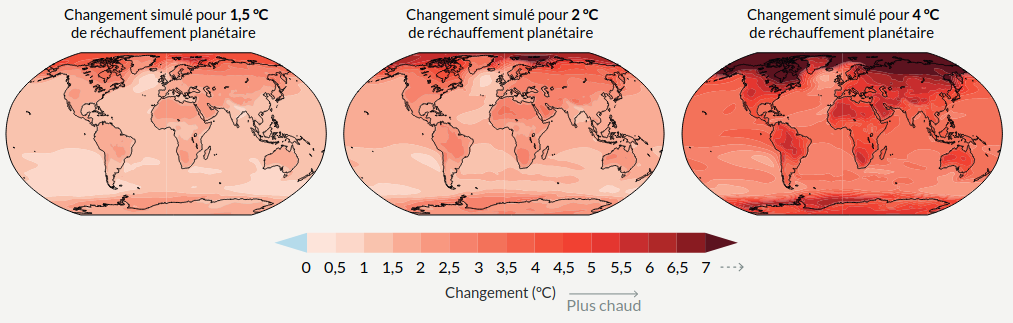
\includegraphics[scale=0.34]{images/Temperature.png}
\\
\tiny{Source : Figure RID.5(b), Résumé à l'intention des décideurs,
 6ème rapport du GIEC, Groupe de travail I}
\end{frame}

\begin{frame}{Plusieurs scénarios possibles}
\centering
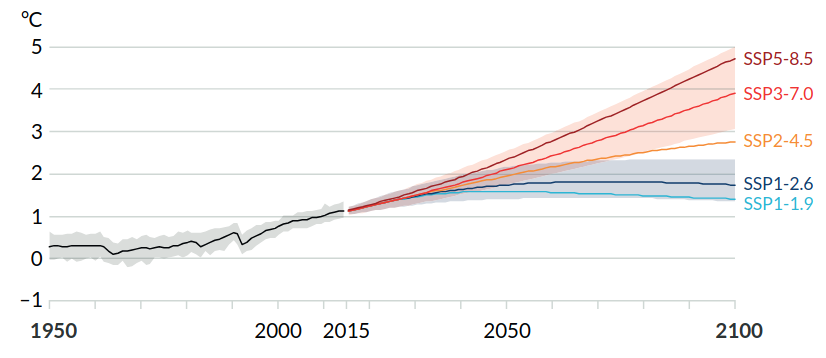
\includegraphics[scale=0.41]{images/IPCC_scenarios.png}
\\
\tiny{Source : Figure RID.8(b), Résumé à l'intention des décideurs,
 6ème rapport du GIEC, Groupe de travail I}
\end{frame}


\begin{frame}{Lien entre GES et température}
\centering
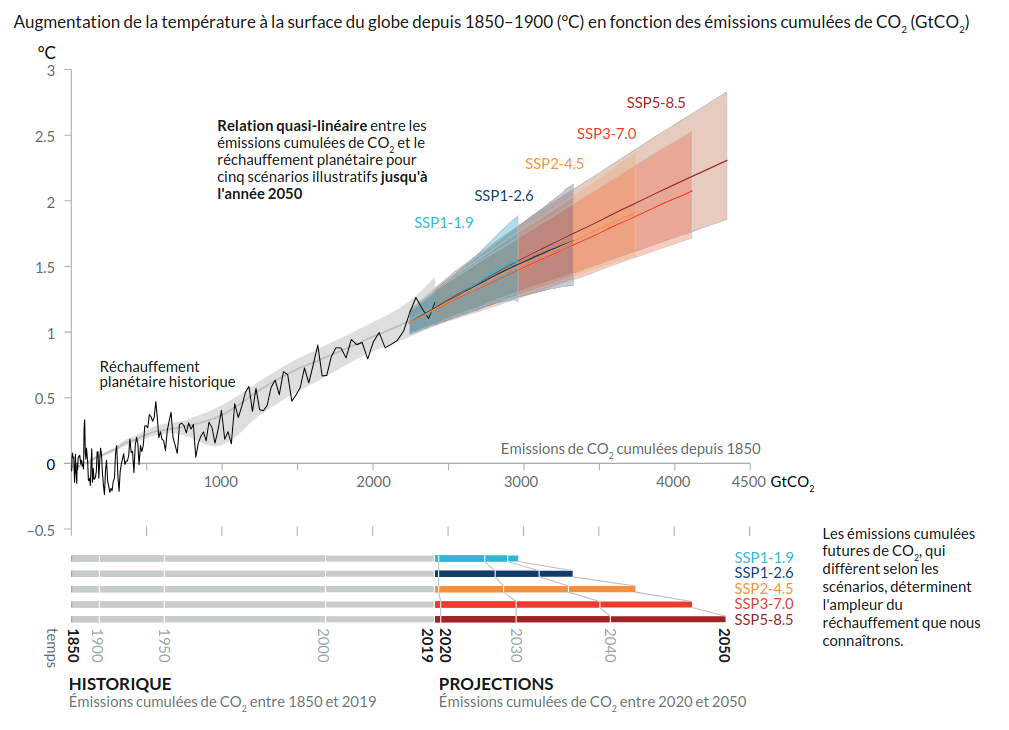
\includegraphics[scale=0.3]{images/Lien_GES_Temperature.png}
\\
\tiny{Source : Figure RID.10, Résumé à l'intention des décideurs,
 6ème rapport du GIEC, Groupe de travail I}
\end{frame}


\begin{frame}
\frametitle{Les 3 groupes de travail du GIEC}

\begin{columns}
  \begin{column}{0.2\textwidth}
Groupe de travail I : 
\end{column}
\begin{column}{0.55\textwidth}
Les bases scientifiques physiques
\end{column}
\begin{column}{0.2\textwidth}
  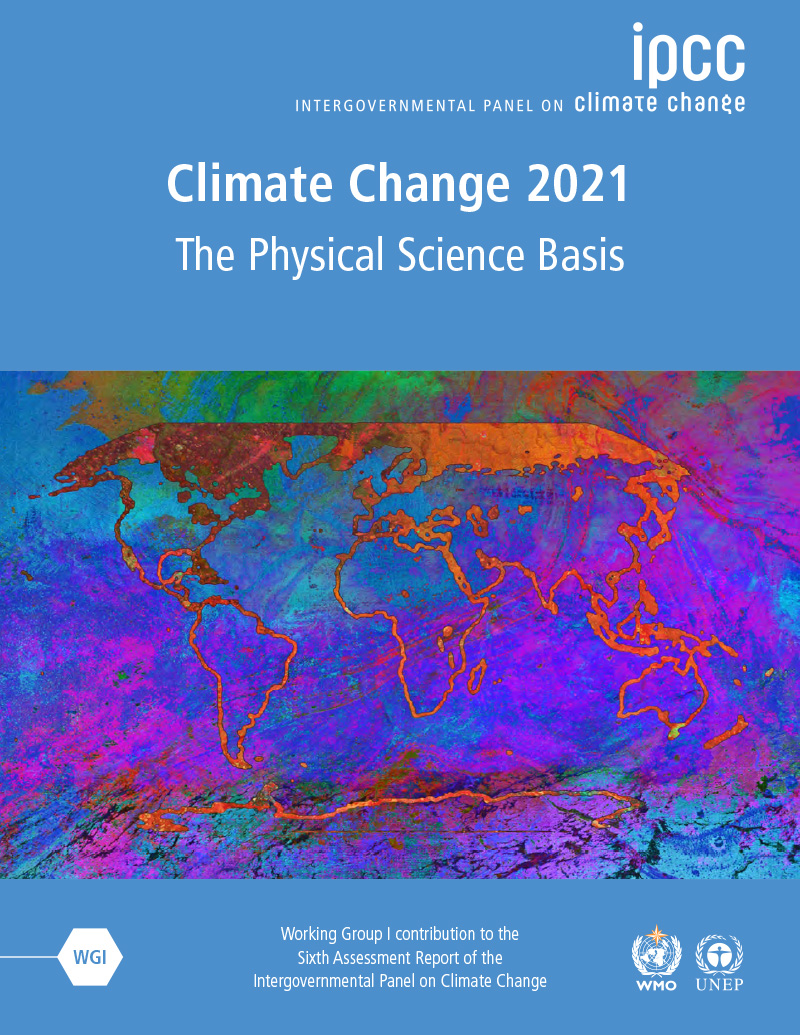
\includegraphics[scale=0.07]{images/IPCC_AR6_WGI.jpg}
\end{column}
\end{columns}
\vspace{0.3cm}
\begin{columns}
  \begin{column}{0.2\textwidth}
Groupe de travail II : 
\end{column}
\begin{column}{0.55\textwidth}
Impacts, adaptation et vulnérabilité
\end{column}
\begin{column}{0.2\textwidth}
  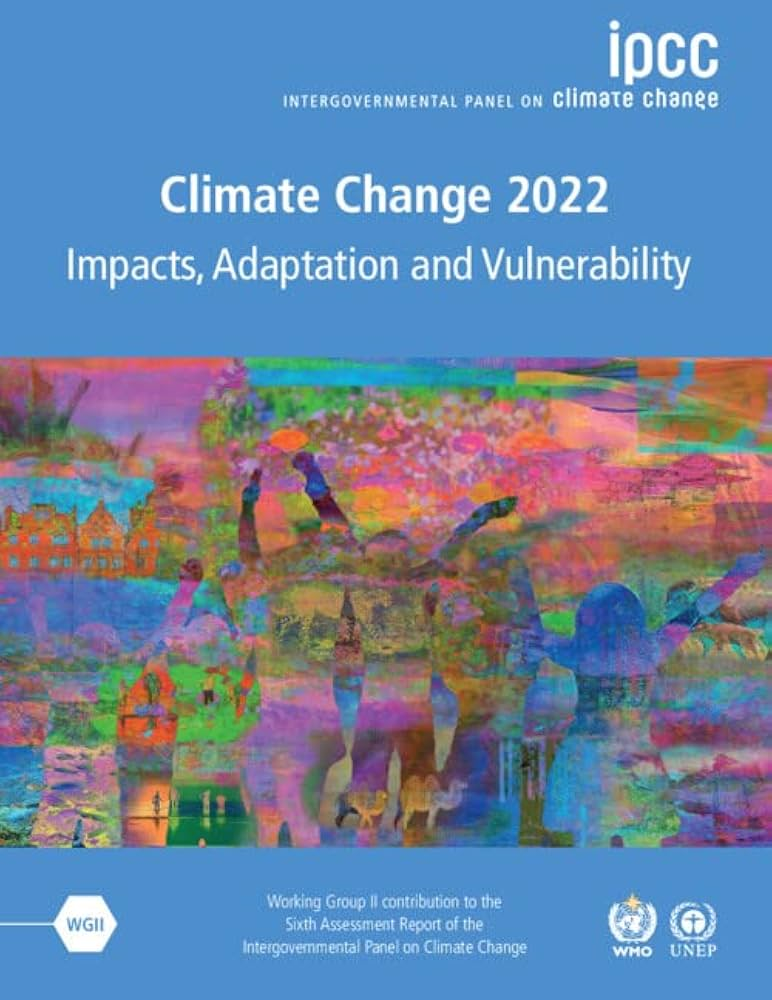
\includegraphics[scale=0.073]{images/IPCC_AR6_WGII.jpg}
\end{column}
\end{columns}
\vspace{0.3cm}
\begin{columns}
  \begin{column}{0.2\textwidth}
Groupe de travail III : 
\end{column}
\begin{column}{0.55\textwidth}
Atténuation du changement climatique
\end{column}
\begin{column}{0.2\textwidth}
  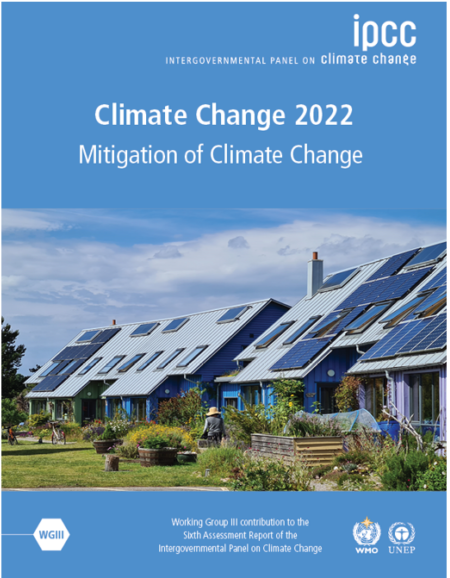
\includegraphics[scale=0.126]{images/IPCC_AR6_WGIII.png}
\end{column}
\end{columns}

\
\end{frame}


\begin{frame}{Groupe 2 : Impacts, adaptation et vulnérabilité}
\centering
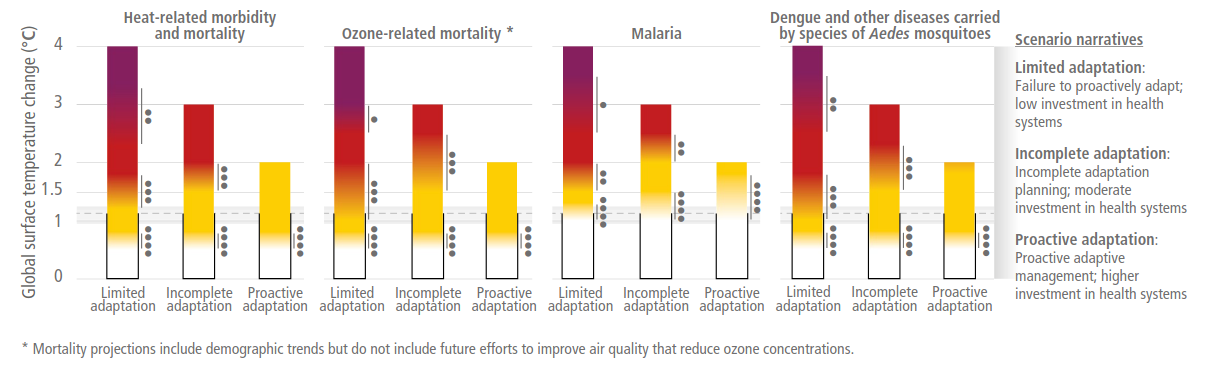
\includegraphics[scale=0.24]{images/Health_adaptation.png}
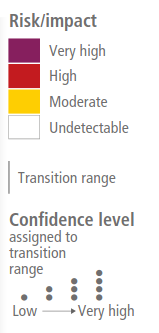
\includegraphics[scale=0.24]{images/Legend_impact_adaptation.png}
\\
\tiny{Source : Figure SPM.3(e), 
 6ème rapport du GIEC, Groupe de travail II}
\end{frame}

\section{Comment compter les émissions de gaz à effet de serre aujourd'hui ?}

\begin{frame}{Potentiel de réchauffement global (PRG)}
\centering
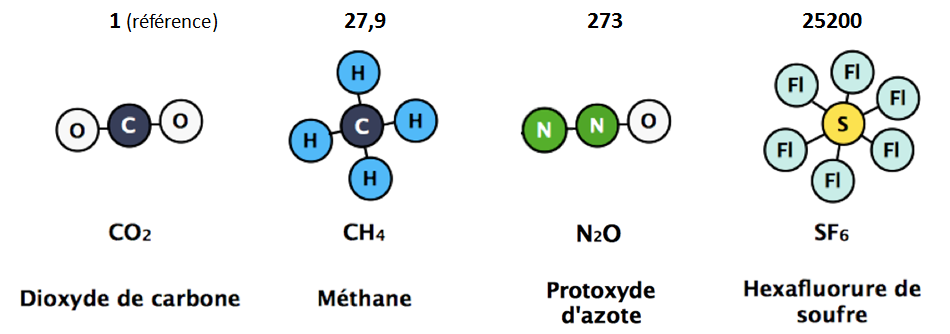
\includegraphics[scale=0.35]{images/PRG.png}
\end{frame}

\begin{frame}{Facteur d'émissions énergies fossiles}
Charbon
Pétrole
Gaz
\end{frame}


\section{Modèles d'évalutions intégrés}
\subsection{Modèles statiques}
\begin{frame}
\frametitle{Équation de Kaya}
\begin{equation*}
GES=POP \times \frac{PIB}{POP} \times \frac{Energie}{PIB}\times \frac{GES}{Energie}
\end{equation*}
\end{frame}

\begin{frame}
\frametitle{Modèle de parc}
\begin{equation*}
GES=\sum_{k \in Logements}POP \times \frac{PIB}{POP} \times \frac{Energie}{PIB}\times \frac{GES}{Energie}
\end{equation*}
\begin{equation*}
GES=\sum_{k \in Vehicules }POP \times \frac{PIB}{POP} \times \frac{Energie}{PIB}\times \frac{GES}{Energie}
\end{equation*}
\end{frame}


 
\subsection{Modèles dynamiques}

\begin{frame}{World 3 et club de Rome}
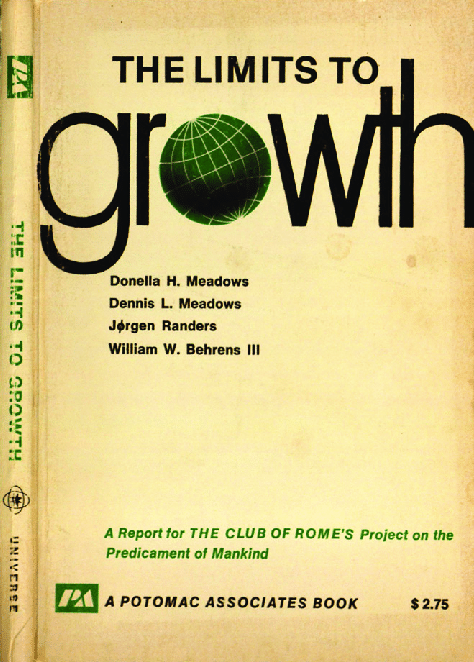
\includegraphics[scale=0.1]{images/limits_to_growth.png}
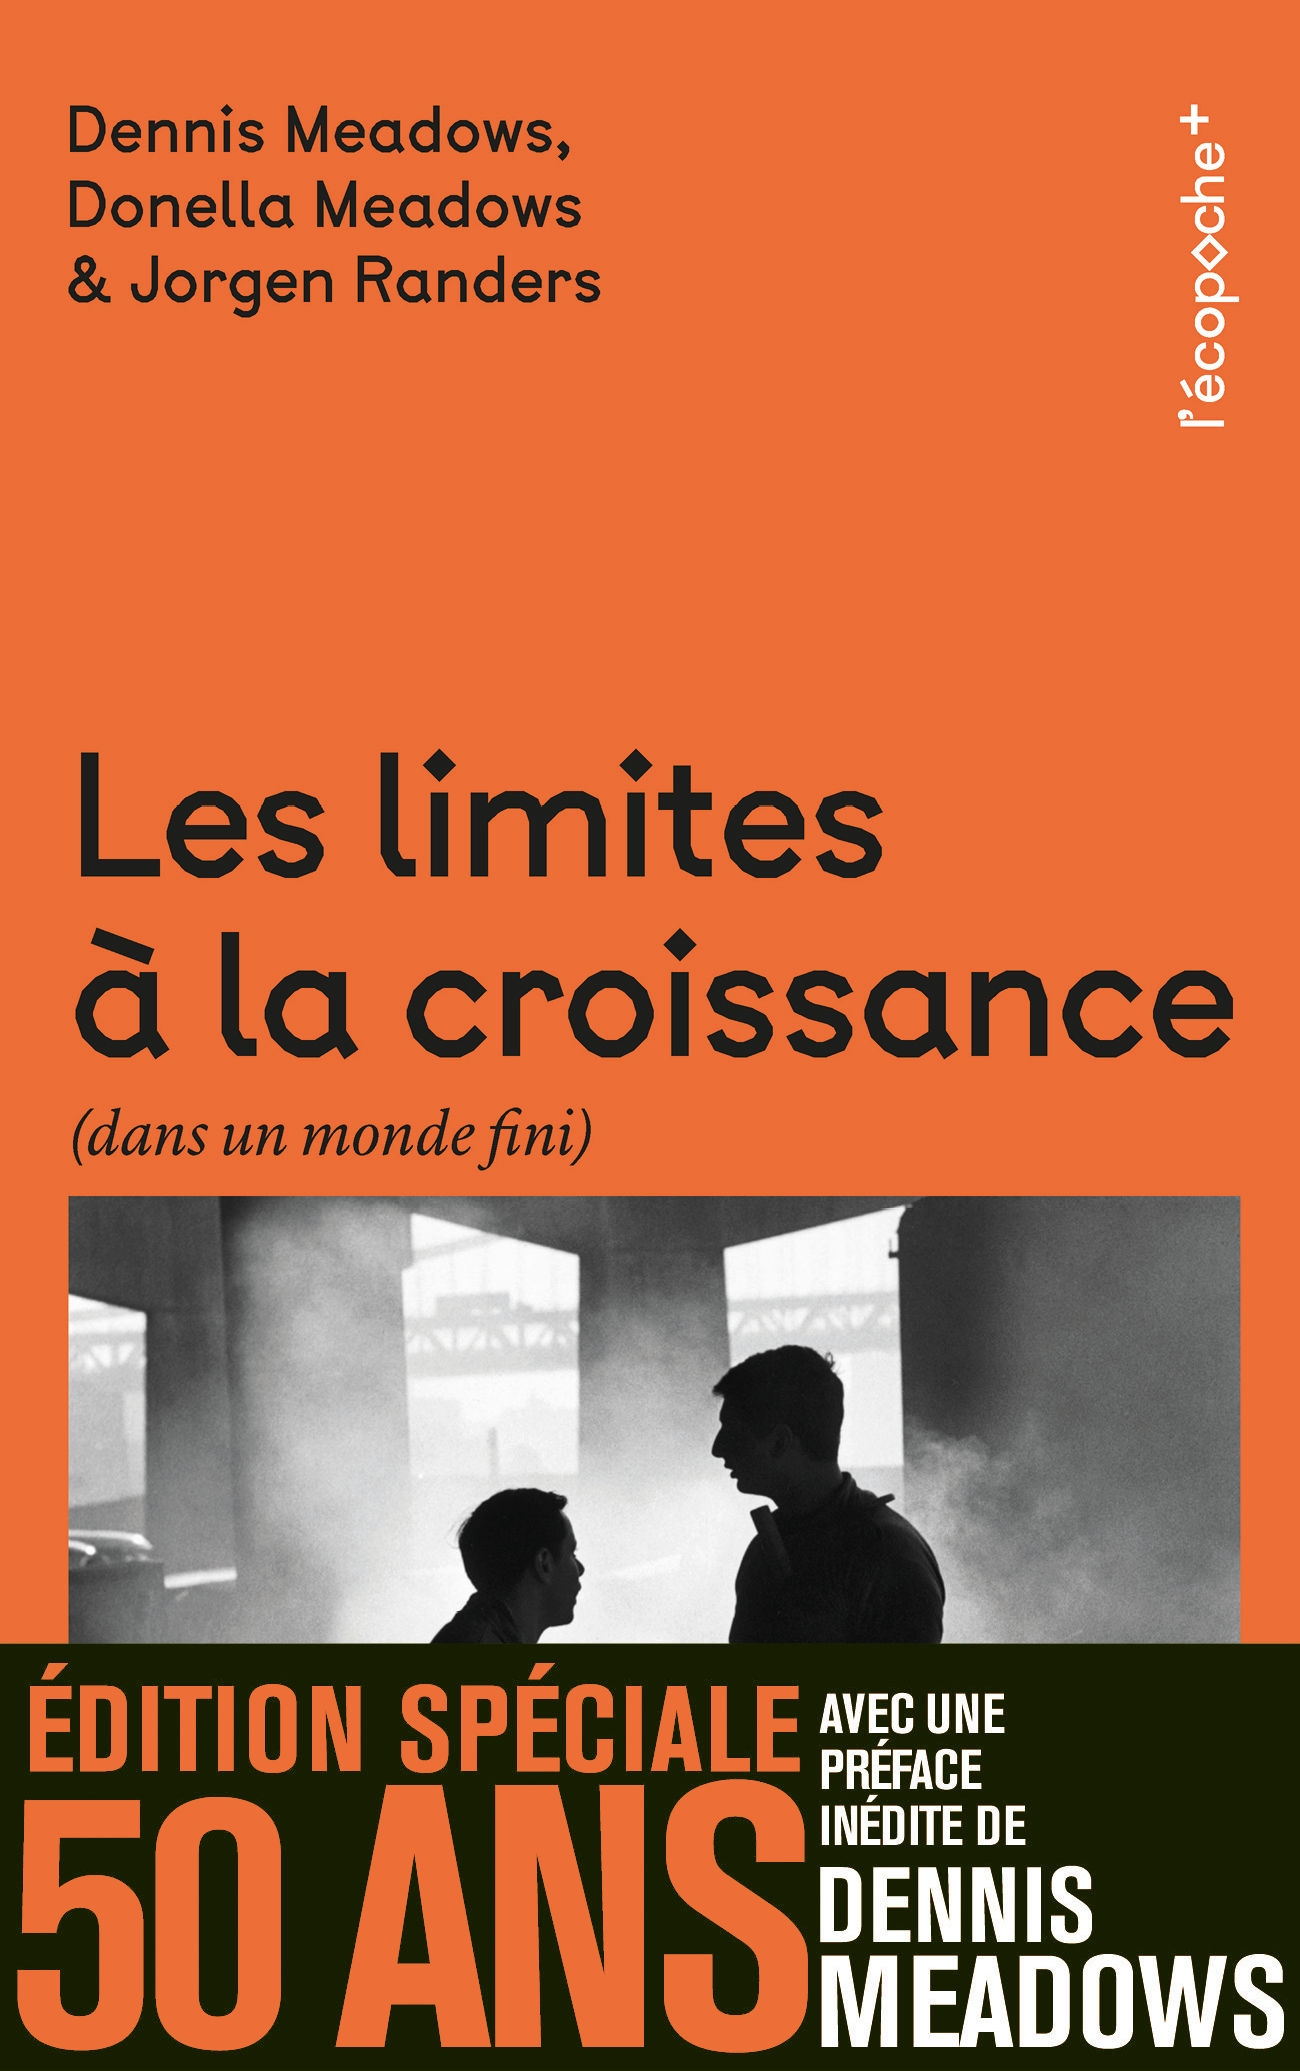
\includegraphics[scale=0.04]{images/limites_croissance.jpg}
\end{frame}

\subsection{Modèles d'optimisation}
\begin{frame}{DICE}
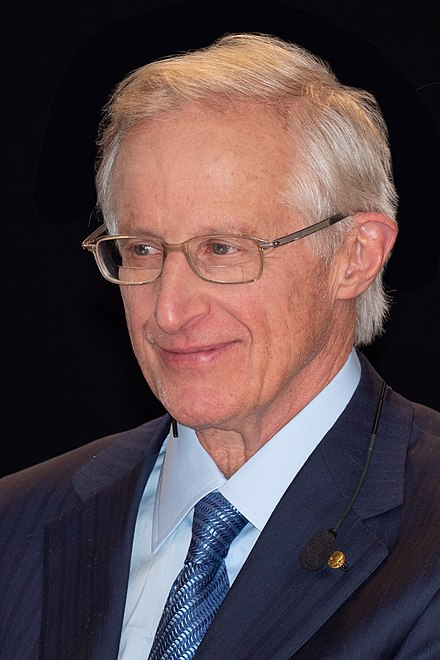
\includegraphics[scale=0.2]{images/Nordhaus.jpg}
\end{frame}



\end{document}